\documentclass[a4paper]{article}

\usepackage[francais]{babel}
\usepackage[utf8x]{inputenc}
\usepackage[T1]{fontenc}
%\usepackage{amsmath}
\usepackage{graphicx}
\usepackage[colorinlistoftodos]{todonotes}
\usepackage{comment}
\usepackage{float}
\usepackage[colorlinks=true,linkcolor=black,citecolor=black]{hyperref}
\usepackage{colortbl}


\title{\bsc{INSA} de Rennes \\ Département Informatique \\ \bigskip \hrule \bigskip ArchiPoilus \\ \bigskip Système d'annotation et de navigation dans des images d'archives \\ \bigskip Dossier de planification initiale \bigskip \hrule}
\author{Raphaël \bsc{Baron}, Pierre-Olivier \bsc{Bouteau}, Nicolas \bsc{Charpentier}, \\ Clément \bsc{Leboullenger}, Thomas \bsc{François}, Benoit \bsc{Travers}}

\begin{document}

\maketitle
\thispagestyle{empty}

\newpage
\tableofcontents
\thispagestyle{empty}

\newpage
\phantomsection
\addcontentsline{toc}{section}{Introduction}
\section*{Introduction}

	Les Archives départementales d'Ille-et-Vilaine sont en charge de la collecte, du classement, de la conservation et de la communication des archives qui constituent une grande partie du patrimoine historique écrit du département. 
\`A l'approche du centenaire de la Première Guerre Mondiale, les Archives, en collaboration avec l'\bsc{INSA} de Rennes, ont choisi de proposer aux étudiants en quatrième année du département informatique un sujet de mise en valeur des documents li\'es \`a la Grande Guerre.\\

	L'objectif du projet est de construire un outil d'annotations semi-auto\-matiques des documents liés au recrutement militaire concernant cette période. L'outil doit permettre à un utilisateur, visiteur des archives, d'associer lecture et annotation du document avec l'image numérisée qui lui correspond. En plus de naviguer et d'annoter les images, l'usager peut utiliser ces annotations pour rechercher des documents, par exemple trouver une personne grâce a son nom.\\
	
	Ce Dossier de planification initiale présente notre projet dans les grandes lignes ainsi que la planifications des tâches à réaliser tout en indiquant les dates consernant les livrables et les soutenances. Il contiendra notamment un premier diagramme de Gantt résumant graphiquement les intéractions et recouvrements temporels des tâches préalablement définies.\\
	
	Ce travail a fait l'objet d'échanges réguliers avec M. Jean-Yves Le Clerc, adjoint au directeur des Archives départementales d’Ille-et-Vilaine, afin de cibler au mieux les besoins auxquels devra répondre notre produit, et Me. Karen Février, chef de projet chez ATOS, qui nous offre un suivi sur l'aspect gestion de projet ainsi que sur la rédaction des documents.

\newpage

\section{Présentation du projet : ArchiPoilus}

\subsection{Sujet}

	Dans le cadre des projets de 4ième année du département informatique, notre objectif est de développer une application permettant d’annoter des registres matricules militaires (RMM) numérisés ainsi que leurs tables associées. Ces annotations doivent être à la fois simples et rapides à créer. Il sera important de pouvoir visualiser des images afin de pouvoir les annoter. De plus, l’application devra permettre à l’utilisateur de facilement rechercher des informations liées à ces annotations. Les principales fonctionnalités à développer seront la recherche de RMM ou d’informations, la visualisation d’images et l’annotation de ces images. Conformément au cahier des charges, notre application sera conçue pour fonctionner sur une table Microsoft PixelSense : nous utiliserons donc des émulateurs pour le développement du projet.\\
	
	Notre équipe est composée de 6 élèves ingénieurs de 4ème année du département informatique de l’INSA de Rennes : Raphaël \bsc{Baron}, Pierre-Olivier \bsc{Bouteau}, Nicolas \bsc{Charpentier}, Clément \bsc{Leboullenger}, Thomas \bsc{François} et Benoit \bsc{Travers}. Nous devons toutefois prendre en compte l’absence de Thomas et Benoit lors du second semestre pour cause de mobilité internationale; l’équipe sera donc réduite à quatre étudiants pour développer le projet pendant cette période.

\subsection{Mise en valeur des documents de guerre}

	L'application étant destinée à être utilisée dans le cadre du centenaire de la guerre 14-18, deux types de documents nous intéressent particulièrement : le registre matricule militaire et la table des registres matricules militaires. Ces documents ont été donnés aux archives par l'armée.

\subsubsection{Le registre matricule militaire}
	Le RMM (Registre Matricule Militaire), dont vous trouverez un exemple complet en annexe \ref{sec:annexe 1}, est un document qui récapitule la carrière d'un soldat. On peut notamment y trouver l'état civil, c'est-à-dire son nom, son prénom, la date et le lieu de sa naissance et les noms de ses parents, ainsi que la description physique du soldat, le lieu de son engagement et ses différentes affectations. On y trouve aussi les campagnes auxquelles il a pris part, ainsi que ses éventuelles décorations et/ou condamnations.

	\`A la lumière du centenaire de la guerre 1914-1918, ces RMM prennent un intérêt particulier. En effet, ils permettent de déterminer quels soldats ont pris part à cette guerre, quelles batailles ils ont menées, et quel destin ils y ont trouvé. En bref, la mise en lumière du centenaire passe en grande partie par la mise en valeur de ces documents, qui seront mis en ligne par les archives d'Ille-et-Vilaine pour l'occasion.\\

	Le Registre Matricule Militaire est le document de base de notre projet. Afin de mieux le comprendre, celui-ci, étant divisé en plusieurs parties, est expliqué plus en détails dans notre rapport de pré-étude.

	Pour le RMM, il devra être possible, à travers l'application, de tout annoter, de n'importe quelle information présente dans le RMM jusqu'à l'annotation personnelle. 

\subsubsection{Les tables des registres matricules militaires}
	La table des RMM représente la liste de tous les registres présents dans un volume. Elle est triée par ordre alphabétique et permet donc de retrouver facilement un RMM, qui sont eux classés par numéros matricules croissants. Vous trouverez un exemple en annexe \ref{sec:annexe 2} où l'on peut trouver le matricule et donc le RMM de l'individu nommé Onen (annexe \ref{sec:annexe 1}).

	Ces tables nous seront utiles pour la rapidité de recherche de l'information. En effet, le numéro matricule est un moyen de recherche efficace puisqu'ils sont rangés, dans un volume, en ordre numérique. 

	L'objectif de l'application sera donc d'offrir la possibilité de naviguer d'une table à un RMM directement en rendant donc la zone du numéro matricule "cliquable" tel un lien hypertexte.

\subsection{Fonctionnalités Générales}

	Parler de l'architecture générale ?????
 
	Pour réaliser l'application nous avons regroupé les différentes fonctionnalitées à développer en six groupes qui sont : l'authentification, la recherche, la navigation, la visualisation des documents, l'annotation de ces documents et la gestion des utilisateurs. 

\subsubsection{Authentification}
\subsubsection{Recherche}
\subsubsection{Navigation}
\subsubsection{Visualisation des documents}
\subsubsection{Annotation}


\subsubsection{Administration}

	Cette fonctionnalité est la moins prioritaire. En effet, notre premier objectif est de réaliser une première version fonctionnelle, c'est-à-dire uniquement avec les fonctionnalités de base. C'est pourquoi, par manque de temps, cette fonctionnalité ne sera pas développée dans un premier temps. Toutefois, nous souhaitons la faire apparaître dans ce rapport car son développement apporterait un vrai plus à l'application.
	
\section{Planification des tâches}

	\subsection{Dates des Soutenances et des Livrables}
	
	Présentation des deadlines à respecter
	
	\subsection{Cycle en V}
	
	Justification par rapport à une méthode agile trop dure à mettre en place car trop peut de temps pour faire itération et rendu des livrables correspond à un cycle en V (!= agile avec plusieurs version d'une application et plusieurs retour des clients (ici les archives peuvent faire client, mais trop peu de temps pour faire plusieurs itérations))
	
	\subsection{Planification des tâches}
	
	(temps de travail par semaine, temps au total = temps prévu, tâches moins importantes, ...)
	(travail sous ms project : Voir avec la nvelle version si une autre visualisation de la planif n'est pas plus intéressante, temps de travail par semaine, semaines particulière)
	

\newpage
\phantomsection
\addcontentsline{toc}{section}{Conclusion}
\section*{Conclusion}

CE RAPPORT EST TROP GENIAAAAAAAAL ! Et moi aussi, en toute modestie...

\appendix

\section{Vue compl\`ete d'un RMM}
\label{sec:annexe 1}

\begin{figure}[H]
\centering
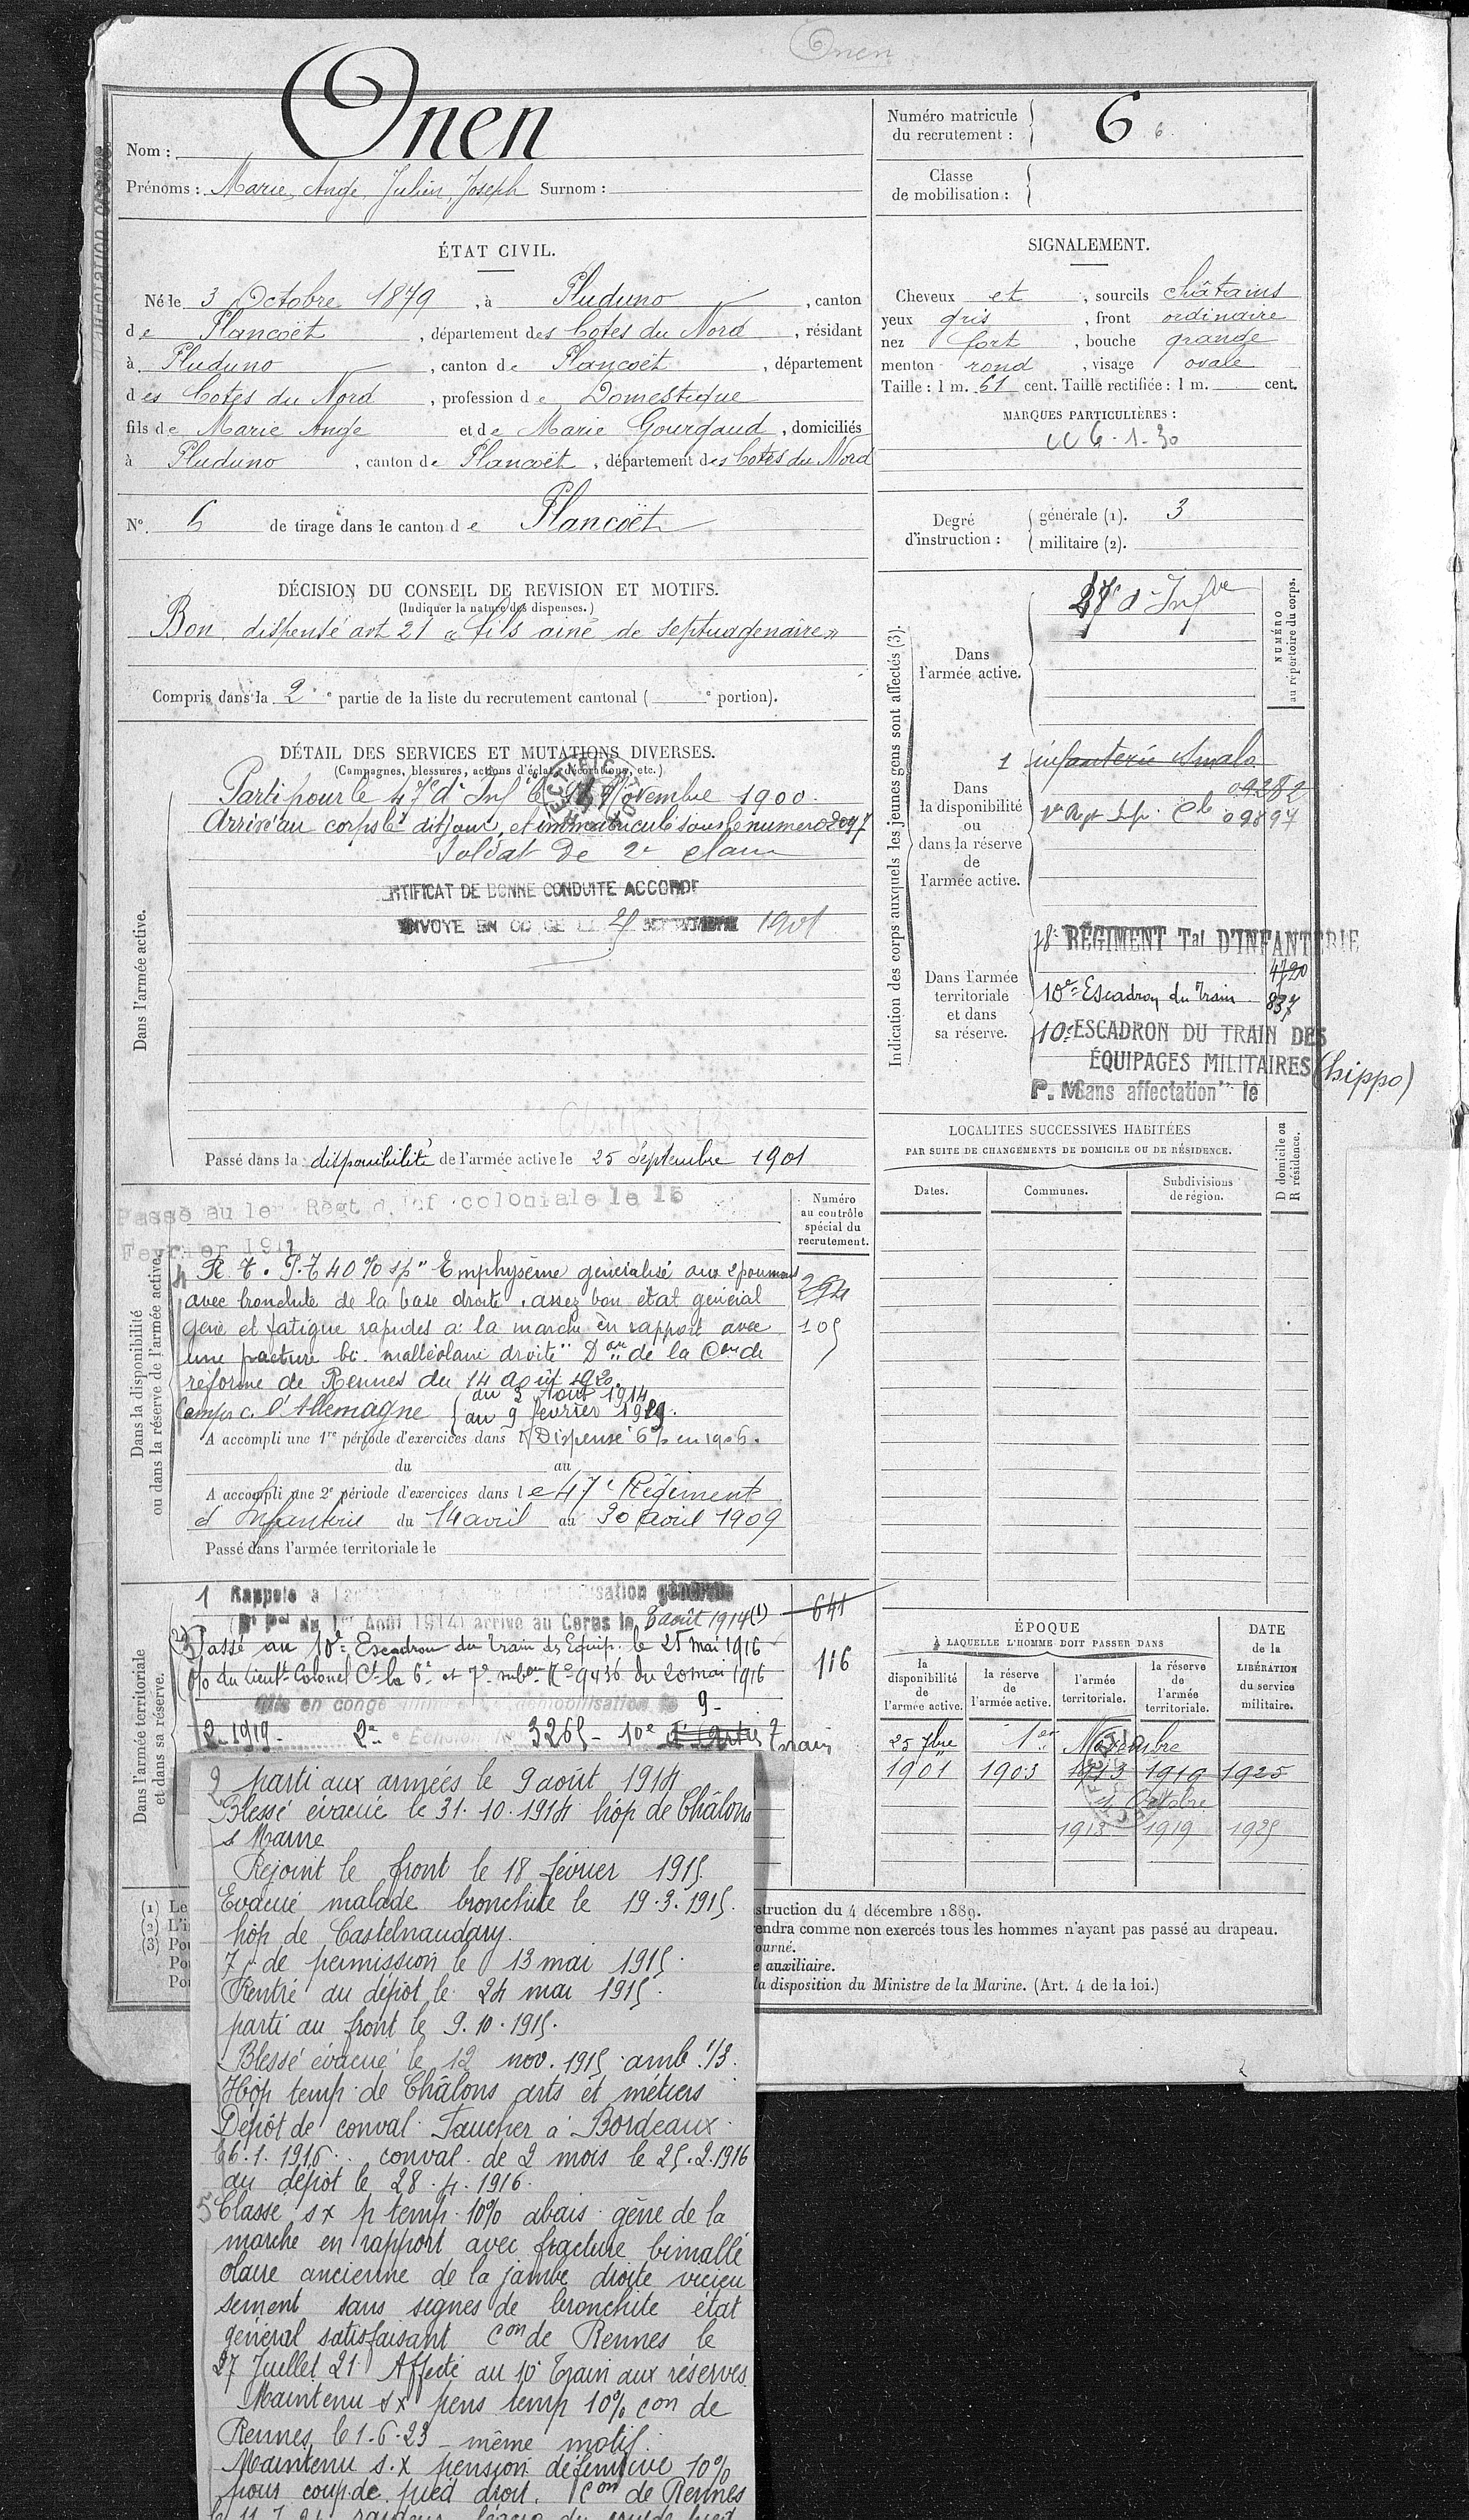
\includegraphics[width=0.95\textwidth]{RMM.JPG}
\end{figure}

\section{Table de RMM - Saint-Malo 1899}
\label{sec:annexe 2}

\begin{figure}[H]
\centering
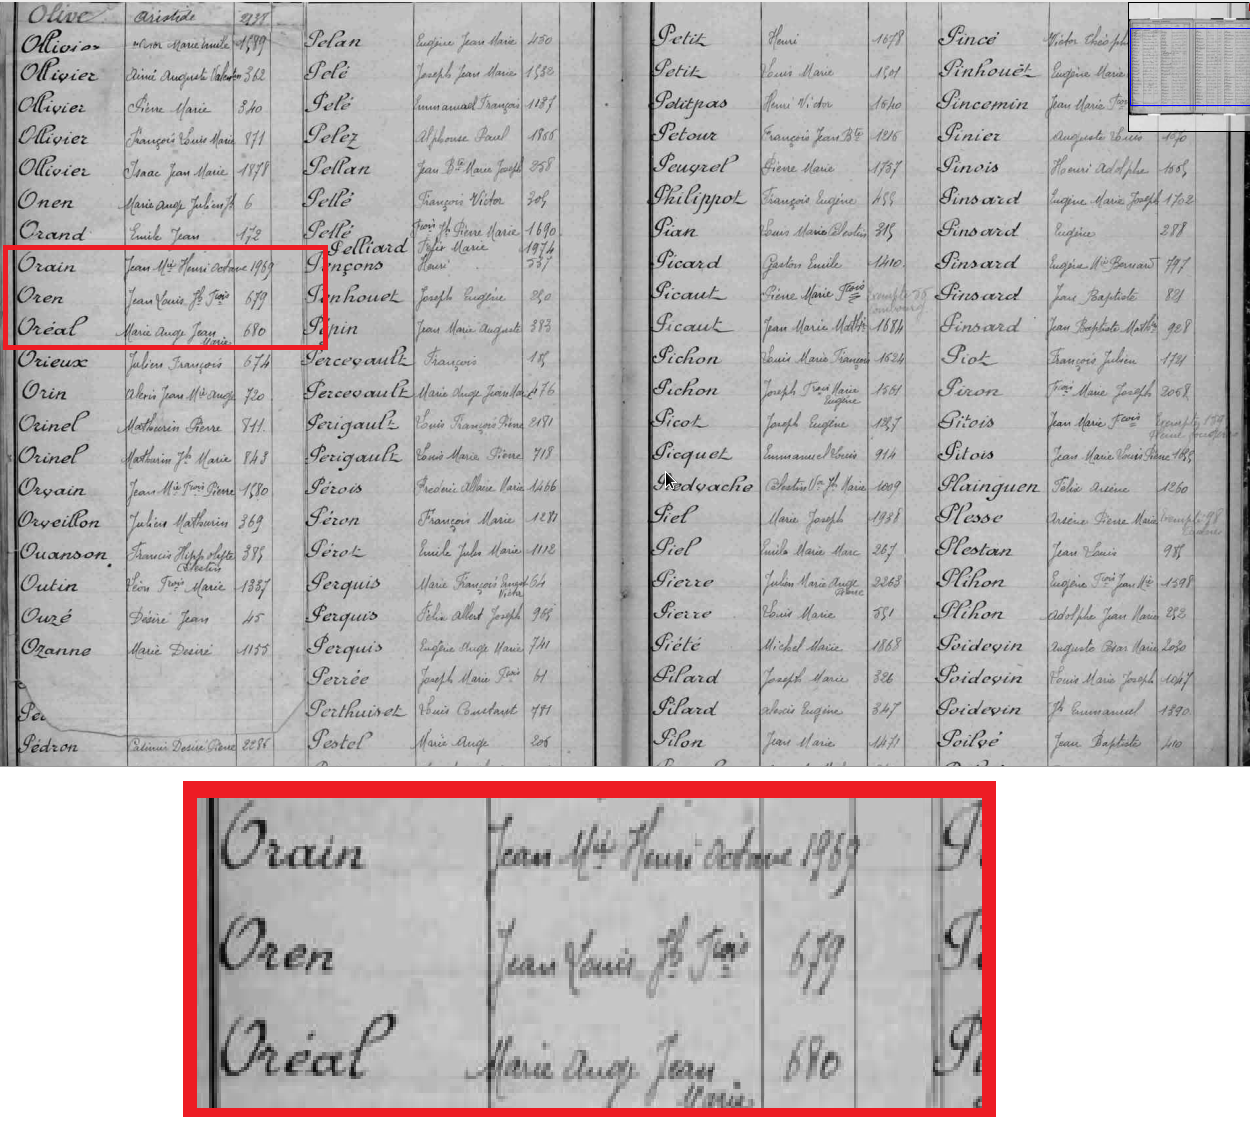
\includegraphics[width=\textwidth]{Table_Onen.png}
\end{figure}

\end{document}
